\chapter{Parallel Architectures}
\label{Chapter2prime}
After establishing a comparative study of the existing, this chapter is meant to define the main features and the architecture of both Hadoop Distributed File System and Apache spark framework.  

\section{The Hadoop Distributed File System}

The Hadoop Distributed File System (HDFS) is a distributed file system designed to run on service hardware. Unlike other distributed systems, HDFS is highly fault-tolerant and designed using low-cost hardware. HDFS holds very large amount of data and provides easier access. To store such huge data, the files are stored across multiple machines. These files are stored in a way to rescue the system from possible data losses in case of failure. HDFS also makes applications available to parallel processing \cite{cite14}.\\

\subsection{Features of HDFS:}
HDFS provides a plenty of functionalities and features that make processing and storing huge datasets easier and more secure. To better understand HDFS, following will explain its goals and assumptions: \\

\textbf{\normalsize{Hardware Failure}}\\

Hardware failure is the norm rather than the exception in HDFS architecture. A node may consist of many server machines, each storing part of the file system's data. The fact that there are a big number of components and that each component has a non-trivial possibility of failure means that some component of HDFS is always non-functional. Thus, quick detection of faults and automatic recovery is a core architectural goal of HDFS.\\

\textbf{\normalsize{Streaming Data Access}}\\

Applications' datasets that run on HDFS need streaming to access. They are not general purpose applications that classically run on general purpose file systems. HDFS is designed more for batch processing rather than interactive use. The emphasis is on high amount of data access rather than low latency of data access. POSIX imposes many hard requirements that are not needed for applications that are targeted for HDFS. POSIX semantics in a few key areas has been traded to rise data throughput rates.\\

\textbf{\normalsize{Large Datasets}}\\

A usual file in HDFS is huge in size. HDFS is designed, then, to support large files. It should provide high aggregate data bandwidth and scale to hundreds of nodes in a single cluster. It should support tens of millions of files in a single instance.\\

\textbf{\normalsize{Simple Coherency Model}}\\

HDFS applications need a "write once read many" access model for files. A file once created, written, and closed needs not to be changed. This assumption simplifies data coherency issues and enables high amount data access. A Map-Reduce application or a web based application fits perfectly with this model. There is a plan to support appending-writes to files in the future.\\

\textbf{\normalsize{Computing Data Mode}}\\

A computation requested by an application is much more efficient if it is executed near the data it operates on. This is especially true when the size of the dataset is huge. This minimizes network congestion and increases the overall throughput of the system. The assumption is that it is often better to migrate the computation closer to where the data is located rather than moving the data to where the application is running. HDFS provides interfaces for applications to move themselves closer to where the data is located.\\

\textbf{\normalsize{Portability Across Hardware and Software Platforms}}\\

HDFS has been designed to be easily portable from one platform to another. This helps extensive adoption of HDFS as a platform of choice for a large number of applications.

 
\subsection{HDFS Architecture:}

HDFS follows the master/slave architecture and it has the following elements. Figure \ref{hdfsarch} given below is the architecture of a Hadoop File System \cite{cite15}.

\begin{figure}[H]
\begin{center}
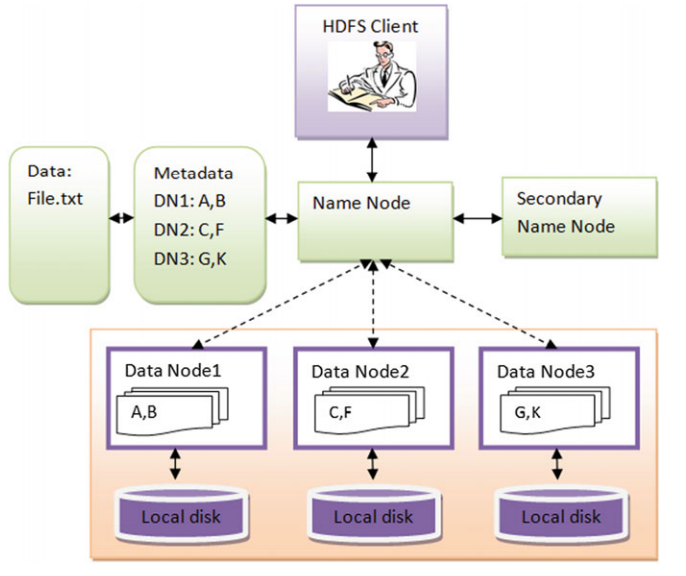
\includegraphics[width=13.8cm,height=8cm]{chapter2/fig2.png}
\end{center}
%légende de l'image
\caption{HDFS Architecture}
\label{hdfsarch}
\end{figure}

\begin{itemize}
\item \textbf{NameNode:} The namenode is the commodity hardware that contains the operating system and the namenode software. It is a software that can be run on commodity hardware. The system having the namenode acts as the master server and it does the following tasks: 
\begin{itemize}
\item Manages the file system namespace.
\item Regulates client's access to files.
\item It also executes file system operations such as renaming, closing, and opening files and directories.
\end{itemize}
A secondary namenode is defined as a backup name node in case of failure.
\item \textbf{DataNodes:} The datanode is a commodity hardware having an operating system and datanode software. For every node (Commodity hardware/System) in a cluster, there will be a datanode. These nodes manage the data storage of their system. 
\begin{itemize}
\item Datanodes perform read-write operations on the file systems, as per client request.
\item They also perform operations such as block creation, deletion, and replication according to the instructions of the namenode. 
\end{itemize}

\item \textbf{Blocks:} Generally the user data is stored in the files of HDFS. The file in a file system will be divided into one or more segments and stored in individual data nodes. These file segments are called as blocks. In other words, the minimum amount of data that HDFS can read or write is called a Block. HDFS configuration set the block size. Otherwise, it will be defined by default.

\item \textbf{HDFS Client:} User applications access the file system using the HDFS client library. HDFS supports operations to read, write and delete files, and operations to create and delete directories. The user references files and directories by paths in the namespace. The user application does not need to know that file blocks are on different servers \cite{cite13}. When an application reads a file, the HDFS client first asks the namenode for the list of datanodes that host blocks replicas of the file. It then contacts a datanode directly and requests the transfer of the desired block. When a client writes, it asks the namenode to choose datanodes to host replicas of the first block of the file. The client organizes a pipeline from node to node and sends the data. When the first block is filled, the client requests new datanodes to be chosen to host replicas of the next block. A new pipeline is organized, and the client sends the further bytes of the file. Each choice of datanodes is likely to be different. The interactions among the client, the namenode and the datanodes are illustrated in figure \ref{interaction}.
\end{itemize} 


\begin{figure}[H]
\begin{center}
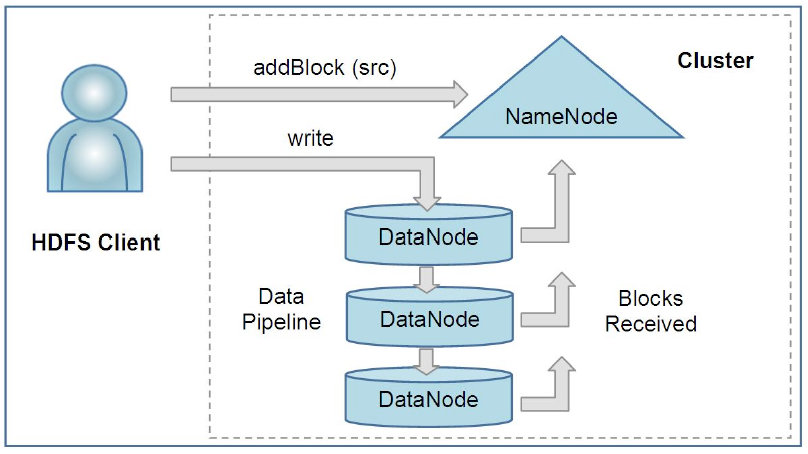
\includegraphics[width=13.5cm,height=6cm]{chapter2/fig1.png}
\end{center}
%légende de l'image
\caption{Interaction between a HDFS Client and Cluster}
\label{interaction}
\end{figure}


\subsection{The File System Namespace}

HDFS supports a traditional hierarchical file organization. A user or an application can create directories and store files inside these directories. The file system namespace hierarchy is similar to most other existing file systems; one can create and remove files, move a file from one directory to another, or rename a file.\\

The namenode maintains the file system namespace. Any change to the file system namespace or its properties is recorded by the namenode. An application can specify the number of replicas of a file that should be maintained by HDFS. The number of copies of a file is called the replication factor of that file. This information is stored by the nameode \cite{cite23}.\\

\subsubsection{File Read and Write}

An application adds data to HDFS by creating a new file and writing the data to it. After the file is closed, the bytes written cannot be altered or removed except that new data can be added to the file by reopening the file for append. HDFS implements a single writer, multiple reader model.\\ 

The HDFS client that opens a file for writing is granted a lease for the file; no other client can write to the file. The writing client periodically renews the lease by sending a heartbeat to the namenode. When the file is closed, the lease is revoked. \\

An HDFS file consists of blocks. When there is a need for a new block, the namenode allocates a block with a unique block ID and determines a list of datanodes to host replicas of the block. The datanodes form a pipeline, the order of which minimizes the total network distance from the client to the last datanode. Bytes are pushed to the pipeline as a sequence of packets. The bytes that an application writes first buffer at the client side. After a packet buffer is filled, the data are pushed to the pipeline. The next packet can be pushed to the pipeline before receiving the acknowledgement for the previous packets. The number of outstanding packets is limited by the outstanding packets window size of the client \cite{cite23}. After data are written to an HDFS file, HDFS does not provide any guarantee that data are visible to a new reader until the file is closed.

\begin{figure}[!h]
\begin{center}
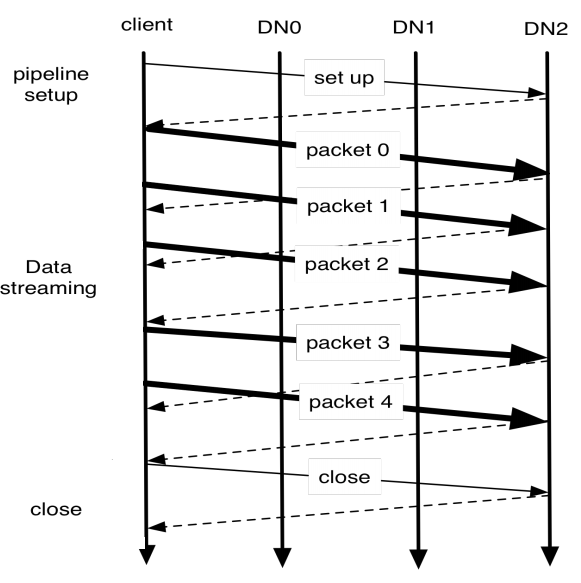
\includegraphics[width=9.5cm,height=9cm]{chapter2prime/pipeline.png}
\end{center}
%légende de l'image
\caption{Data Pipeline During Block Construction}
\label{pipline}
\end{figure}

If no error occurs, block construction goes through three stages as shown in figure \ref{pipline} illustrating a pipeline of three datanodes and a block of five packets. In the picture, bold lines represent data packets, dashed lines represent acknowledgment messages, and thin lines represent control messages to setup and close the pipeline. Vertical lines represent
activity at the client and the three datanodes where time proceeds from top to bottom.\\

When a client opens a file to read, it fetches the list of blocks and the locations of each block replica from the
namenode. The locations of each block are ordered by their distance from the reader. When reading the content of a block,
the client tries the closest replica first. If the read attempt fails, the client tries the next replica in sequence. A read may fail if the target datanode is unavailable, the node no longer hosts a replica of the block, or the replica is found to be corrupt when checksums are tested. HDFS permits a client to read a file that is open for writing. When reading a file open for writing, the length of the last
block still being written is unknown to the namenode. In this case, the client asks one of the replicas for the latest length before
starting to read its content \cite{cite23}.\\


\subsubsection{Replica Placement}
The placement of replicas is critical to HDFS reliability and performance. Optimizing replica placement distinguishes HDFS from most other distributed file systems. The purpose of a rack-aware replica placement policy is to improve data reliability, availability, and network bandwidth utilization.\\

Large HDFS instances run on a cluster of computers that commonly spread across many racks. Communication between two nodes in different racks has to go through switches. In most cases, network bandwidth between machines in the same rack is greater than network bandwidth between machines in different racks.\\

The namenode determines the rack ID each datanode belongs to. A simple policy is to place replicas on unique racks. This prevents losing data when an entire rack. This policy evenly distributes replicas in the cluster, which makes it easy to balance load on component failure. However, this policy increases the cost of writes because a write needs to transfer blocks to multiple racks.
\subsubsection{Communication Protocols}
All HDFS communication protocols are layered on top of the TCP/IP protocol. A client
establishes a connection to a configurable TCP port on the namenode machine. It talks
the ClientProtocol with the namenode. The datanodes talk to the namenode using the
datanode Protocol. A Remote Procedure Call (RPC) abstraction wraps both the Client
Protocol and the datanode Protocol. By design, the namenode never initiates any RPCs. Instead, it only responds to RPC requests issued by datanodes or clients.

\section{Spark: Framework for Parallel Execution}
Apache Spark is a lightning-fast cluster computing technology, designed for fast computation. It is based on Hadoop Map-Reduce and it extends the Map-Reduce model to efficiently use it for more types of computations, which includes interactive queries and stream processing. The main feature of Spark is its in-memory cluster computing that increases the processing speed of an application.\\

Spark is designed to cover a wide range of workloads such as batch applications, iterative algorithms, interactive queries and streaming. Apart from supporting all these workload in a respective system, it reduces the management burden of maintaining separate tools.\\

\subsection{Features of Spark Apache}
\begin{itemize}
\item \textbf{Speed:} Spark helps to run an application in Hadoop cluster, up to 100 times faster in memory, and 10 times faster when running on disk. This is possible by reducing number of read/write operations to disk. It stores the intermediate processing data in memory.
\item \textbf{Supports multiple languages:} Spark provides built-in APIs in Java, Scala, or Python. Therefore, we can write applications in different languages. Spark comes up with 80 high-level operators for interactive querying.
\item \textbf{Advanced Analytics:} Spark not only supports "Map" and "Reduce". It also supports SQL queries, Streaming data, Machine learning (ML), and Graph algorithms.\\
\end{itemize}

\subsection{Components of Spark}

Figure \ref{component} shows the different components of Spark \cite{cite1}.

\begin{figure}[!ht]
\begin{center}
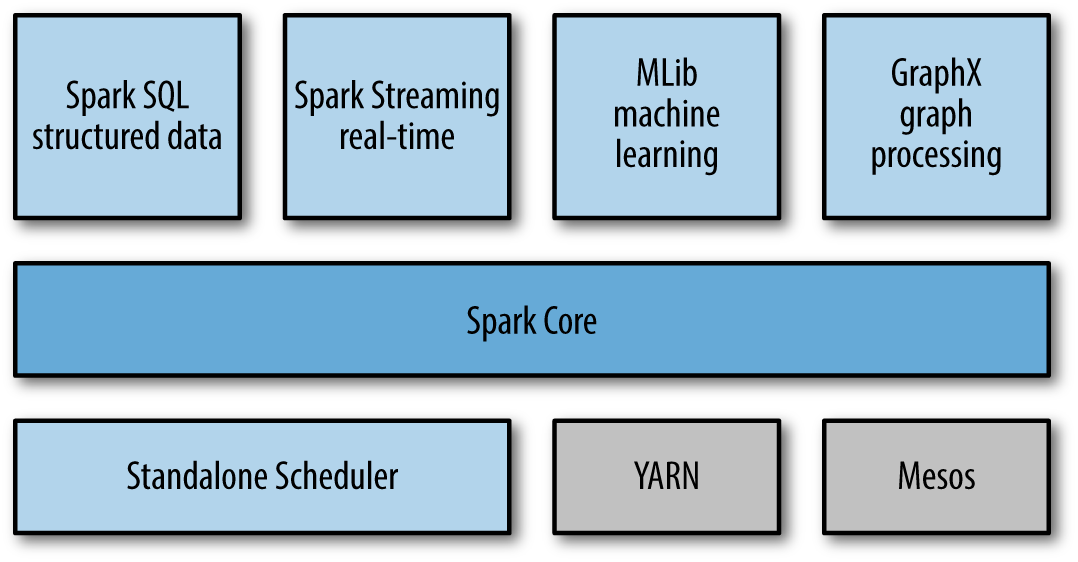
\includegraphics[width=13cm,height=5cm]{chapter2/fig3.png}
\end{center}
%légende de l'image
\caption{The Spark Stack}
\label{component}
\end{figure}



\begin{itemize}
\item \textbf{Apache Spark Core:} Spark Core is the underlying general execution engine for spark platform that all other functionality is built upon. It provides In-Memory computing and referencing datasets in external storage systems.
\item \textbf{Spark SQL:} Spark SQL is a component on top of Spark Core that introduces a new data abstraction called SchemaRDD, which provides support for structured and semi-structured data.
\item \textbf{Spark Streaming:} Spark Streaming leverages Spark Core's fast scheduling capability to perform streaming analytics. It ingests data in mini-batches and performs RDD (Resilient Distributed Datasets) transformations on those mini-batches of data.
\item \textbf{MLlib (Machine Learning Library):} MLlib is a distributed machine learning framework above Spark because of the distributed memory-based Spark architecture. Spark MLlib is nine times as fast as the Hadoop disk-based version.
\item \textbf{GraphX:} GraphX is a distributed graph-processing framework on top of Spark. It provides an API for expressing graph computation that can model the user-defined graphs by using Pregel abstraction API. It also provides an optimized runtime for this abstraction.\\
\end{itemize}

\subsection{Resilient Distributed Datasets}

Resilient Distributed Datasets (RDD) is a fundamental data structure of Spark. It is an immutable distributed collection of objects. Each dataset in RDD is divided into logical partitions, which may be computed on different nodes of the cluster. RDDs can contain any type of Python, Java, or Scala objects, including user-defined classes \cite{cite1}.\\

Formally, an RDD is a read-only, partitioned collection of records. RDDs can be created through deterministic operations on either data on stable storage or other RDDs. RDD is a fault-tolerant collection of elements that can be operated on in parallel. There are two ways to create RDDs: parallelizing an existing collection in the driver program, or referencing a dataset in an external storage system, such as a shared file system, HDFS, HBase, or any data source offering a Hadoop Input Format.\\

Spark makes use of the concept of RDD to achieve faster and efficient MapReduce operations. Let us first discuss how MapReduce operations take place and why they are not so efficient.

\subsection{Map Reduce} 

Map-Reduce is a technique that is widely adopted for processing and generating large datasets with a parallel, distributed algorithm on multiple clusters. It allows users to write parallel computations, using a set of high-level operators, without having to worry about work distribution and fault tolerance.\\

Unfortunately, in most current frameworks, the only way to reuse data between computations is to write it to an external stable storage system. Although this framework provides numerous abstractions for accessing a cluster's computational resources, users still want more.\\

Both Iterative and Interactive applications require faster data sharing across parallel jobs. Data sharing is slow in Map-Reduce due to replication, serialization, and disk input/output (IO). Regarding storage system, most of the Hadoop applications, they spend most of the time doing HDFS read-write operations.
\begin{itemize}
\item \textbf{Iterative Operations on Map Reduce:} Reuse intermediate results across multiple computations in multi-stage applications. Figure \ref{iterative} explains how the current framework works, while doing the iterative operations on Map-Reduce. This incurs substantial overheads due to data replication, disk IO, and serialization, which makes the system slow.

\begin{figure}[H]
\begin{center}
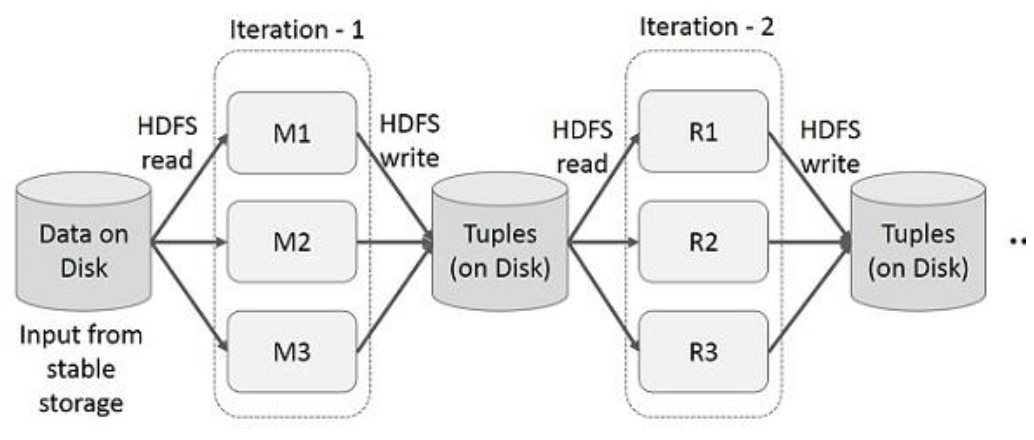
\includegraphics[width=14cm,height=6cm]{chapter2/fig4.png}
\end{center}
%légende de l'image
\caption{Iterative Operations on MapReduce}
\label{iterative}
\end{figure}

\item \textbf{Interactive Operations on MapReduce:} User runs ad-hoc queries on the same subset of data. Each query will do the disk I/O on the stable storage, which can dominates application execution time. Figure \ref{interactive} explains how the current framework works while doing the interactive queries on MapReduce.

\begin{figure}[H]
\begin{center}
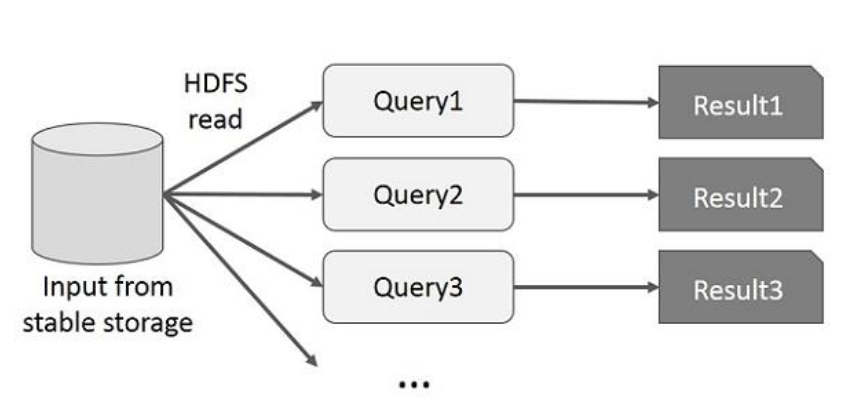
\includegraphics[width=14cm,height=6cm]{chapter2/fig5.png}
\end{center}
%légende de l'image
\caption{Interactive operations on MapReduce}
\label{interactive}
\end{figure}

\item \textbf{Data Sharing using Spark RDD:} Data sharing is slow in Map-Reduce due to replication, serialization, and disk IO. Most of the Hadoop applications, they spend most of the time doing HDFS read-write operations. Recognizing this problem, researchers developed a specialized framework called Apache Spark. The key idea of spark is Resilient Distributed Datasets (RDD); it supports in-memory processing computation. This means, it stores the state of memory as an object across the jobs and the object is sharable between those jobs. Data sharing in memory is 10 to 100 times faster than network and Disk.
Let us now try to find out how iterative and interactive operations take place in Spark RDD.

\item \textbf{Iterative Operations on RDD Spark:} Figure \ref{RDD1} shows the iterative operations on Spark RDD. It will store intermediate results in a distributed memory instead of Stable storage (Disk) and make the system faster.



\begin{figure}[H]
\begin{center}
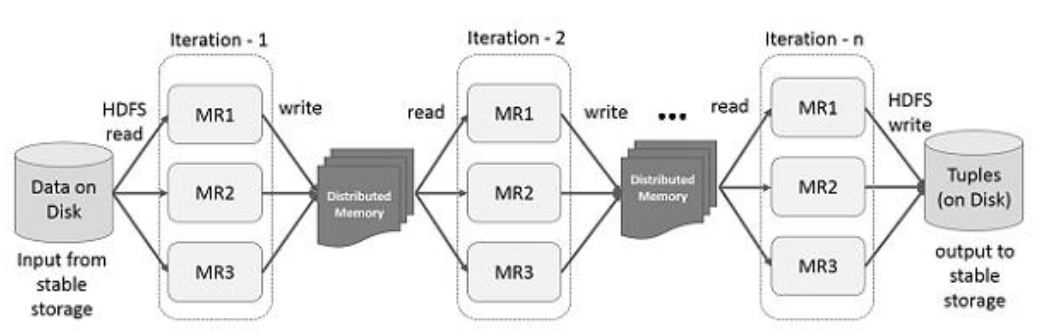
\includegraphics[width=16cm,height=6.5cm]{chapter2/fig6.png}
\end{center}
%légende de l'image
\caption{Iterative operations on Spark RDD}
\label{RDD1}
\end{figure}



\item \textbf{Interactive Operation on Spark RDD:} Figure \ref{RDD2} shows interactive operations on Spark RDD. If different queries are run on the same set of data repeatedly, this particular data can be kept in memory for better execution times.\\

\begin{figure}[H]
\begin{center}
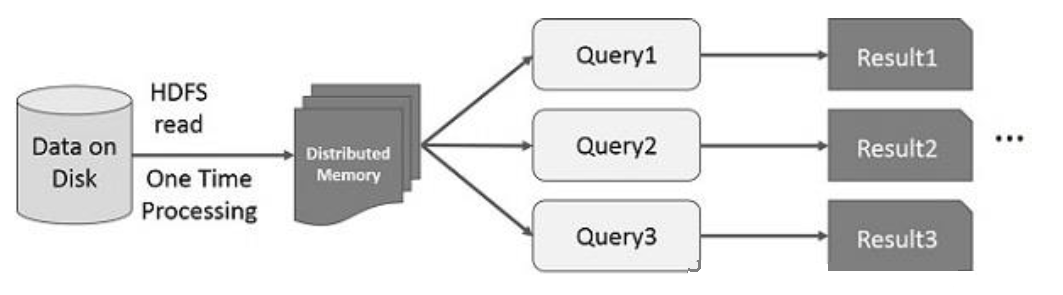
\includegraphics[width=14cm,height=6cm]{chapter2/fig7.png}
\end{center}
%légende de l'image
\caption{Interactive operations on Spark RDD}
\label{RDD2}
\end{figure}

\end{itemize}

\subsection{Spark Architecture}

Spark applications run as independent sets of processes on a cluster, coordinated by a SparkContext object in a main program called the driver program. Specifically, to run on a cluster, the SparkContext can connect to several types of cluster managers; either Spark's own standalone cluster manager, Mesos or YARN, which allocate resources across applications. Once connected, Spark acquires executors on nodes in the cluster, which are processes that run computations and store data for the application. Next, it sends the application code to the executors. Finally, SparkContext sends tasks to the executors to run. Figure \ref{driver} shows how this architecture works.\\
\begin{figure}[!ht]
\begin{center}
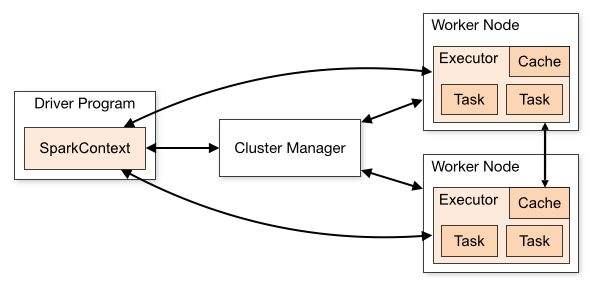
\includegraphics[width=14cm,height=7cm]{chapter2/fig8.png}
\end{center}
%légende de l'image
\caption{Spark Architecture}
\label{driver}
\end{figure}

There are several useful things to note about this architecture:\\
\begin{itemize}
\item Each application gets its own executor processes, which stay up for the duration of the whole application and run tasks in multiple threads. This has the benefit of isolating applications from each other, on both the scheduling side (each driver schedules its own tasks) and executor side (tasks from different applications run in different JVMs). However, it also means that data cannot be shared across different Spark applications (instances of SparkContext) without writing it to an external storage system.
\item Spark is agnostic to the underlying cluster manager. As long as it can acquire executor processes, and these communicate with each other, it is relatively easy to run it even on a cluster manager that also supports other applications.
\item The driver program must listen for and accept incoming connections from its executors throughout its lifetime. As such, the driver program must be network addressable from the worker nodes.
\item Because the driver schedules tasks on the cluster, it should be run close to the worker nodes, preferably on the same local area network. If we'd like to send requests to the cluster remotely, it's better to open an RPC to the driver and have it submit operations from nearby than to run a driver far away from the worker nodes.
\end{itemize}

\section*{Conclusion}

After describing, theoretically, our chosen big data manufacturing tools, in the next
chapter, we are going to start the application development step by, first specifying the requirements of the application that we opt to implement.